\chapter{Matriisit}

Matriisi on kaksiulotteinen taulukko,
jolle on määritelty laskutoimituksia.
Tässä luvussa näemme, miten matriisien
avulla voi optimoida dynaamista ohjelmointia.
Osoittautuu, että jos dynaamisen ohjelmoinnin rekursiossa
lasketaan yhteen kiinteä määrä aiempia arvoja
vakiokertoimilla,
ratkaisun aikavaativuuden saa muutettua lineaarisesta
logaritmisesta matriisien avulla.

\section{Määritelmiä}

Matriisi (\textit{matrix}) on
kaksiulotteista taulukkoa
vastaava matemaattinen käsite.
Esimerkiksi seuraavassa on $3 \times 4$ -kokoinen
matriisi $A$:

\[ A = \left( \begin{array}{ccccc}
8 & 17 & 7 & 4 \\
7 & 19 & 5 & 10 \\
19 & 9 & 4 & 18 \end{array} \right)\] 

Merkitään $A_{i,j}$ matriisin $A$ rivillä $i$
sarakkeessa $j$ olevaa arvoa.
Esimerkiksi yllä olevassa matriisissa
$A_{2,3}=5$.

\subsubsection*{Yhteenlasku}

Matriisien $A$ ja $B$ yhteenlasku $A+B$ on määritelty,
jos kummankin matriisin korkeus ja leveys on sama.
Tällöin uusi matriisi saadaan laskemalla
yhteen kaikki matriisien vastaavissa kohdissa olevat luvut.

Seuraavassa on esimerkki
matriisien yhteenlaskusta:

\[
A = \left( \begin{array}{ccc}
6 & 1 & 4 \\
3 & 9 & 2 \end{array} \right)
\hspace{20px}
B = \left( \begin{array}{ccc}
4 & 9 & 3 \\
8 & 1 & 3 \end{array} \right)
\]
~\\
\[
A+B = 
\left( \begin{array}{ccc}
6+4 & 1+9 & 4+3 \\
3+8 & 9+1 & 2+3 \end{array} \right)
=
\left( \begin{array}{ccc}
10 & 10 & 7 \\
11 & 10 & 5 \end{array} \right)
\] 

\subsubsection*{Kertolasku}

Matriisien $A$ ja $B$ kertolasku $AB$ on määritelty,
jos vasemman matriisin leveys on sama kuin
oikean matriisin korkeus.
Toisin sanoen matriisin $A$ koon tulee olla $a \times n$
ja matriisin $B$ koon tulee olla $n \times b$.
Kertolaskun tuloksena on uusi matriisi,
jonka koko on $a \times b$.

Matriisien kertolaskussa jokainen tulosmatriisin
luku muodostuu summana $A$:n ja $B$:n
lukuparien tuloista.
Summa muodostuu seuraavan kuvan tapaan:
\\
\begin{center}
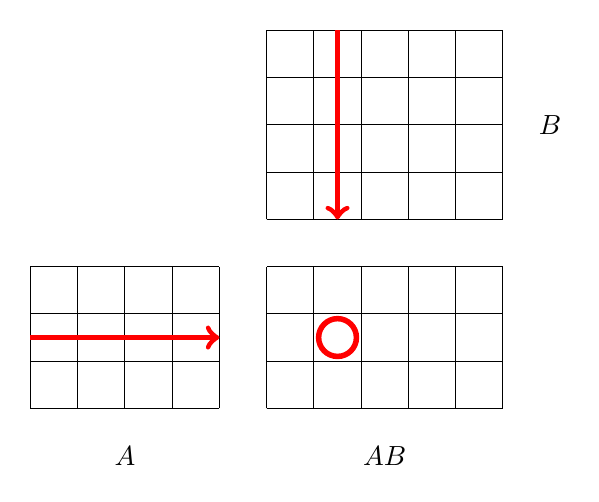
\begin{tikzpicture}[scale=0.6]
\draw (0,0) grid (4,3);
\draw (5,0) grid (10,3);
\draw (5,4) grid (10,8);

\node at (2,-1) {$A$};
\node at (7.5,-1) {$AB$};
\node at (11,6) {$B$};

\draw[thick,->,red,line width=2pt] (0,1.5) -- (4,1.5);
\draw[thick,->,red,line width=2pt] (6.5,8) -- (6.5,4);
\draw[thick,red,line width=2pt] (6.5,1.5) circle (0.4);
\end{tikzpicture}
\end{center}

Kertolaskun matemaattinen määritelmä on:
\[
(AB)_{i,j} = \sum_{k=1}^n A_{i,k} B_{k,j}
\]

Seuraavassa on esimerkkejä matriisien kertolaskuista:
\[
A = \left( \begin{array}{cc}
1 & 4 \\
3 & 9 \\
8 & 6 \end{array} \right)
\hspace{20px}
B = 
\left( \begin{array}{cc}
1 & 6 \\
2 & 9 \end{array} \right)
\]
\[
AB =
\left( \begin{array}{ccc}
1 \cdot 1 + 4 \cdot 2 & 1 \cdot 6 + 4 \cdot 9 \\
3 \cdot 1 + 9 \cdot 2 & 3 \cdot 6 + 9 \cdot 9 \\
8 \cdot 1 + 6 \cdot 2 & 8 \cdot 6 + 6 \cdot 9 \end{array} \right)
=
\left( \begin{array}{ccc}
9 & 42 \\
21 & 99 \\
20 & 102 \end{array} \right)
\] 

\[
A = \left( \begin{array}{ccc}
9 & 6 & 5 \\
4 & 1 & 8 \end{array} \right)
\hspace{20px}
B = \left( \begin{array}{c}
3 \\
5 \\
8 \end{array} \right)
\]
\[
AB =
\left( \begin{array}{c}
9 \cdot 3 + 6 \cdot 5 + 5 \cdot 8 \\
4 \cdot 3 + 1 \cdot 5 + 8 \cdot 8 \end{array} \right)
=
\left( \begin{array}{ccc}
97 \\
81 \end{array} \right)
\] 

Tavallisesta kertolaskusta poiketen matriisien
kertolasku ei ole vaihdannainen,
eli ei ole voimassa $AB = BA$.
Kuitenkin matriisien kertolasku
on liitännäinen eli
on voimassa $A(BC)=(AB)C$.

Matriisikertolaskun aikavaativuus kolmea for-silmukkaa
käyttäen on $O(n^3)$, kun matriisin koko on $n \times n$.

\subsubsection*{Potenssilasku}

Matriisien potenssilasku määritellään
saman tapaan kuin tavallinen potenssilasku,
esimerkiksi $A^3=AAA$.

Potenssilaskun $A^k$ aikavaativuus on $O(n^3 k)$,
jos sen toteuttaa $k$ kertolaskuna.
Mutta potenssilaskun voi toteuttaa
myös ajassa $O(n^3 \log k)$ tehokkaalla
potenssilaskulla (luku 21.2).

Esimerkiksi lasku
\[
\left( \begin{array}{cc}
1 & 4 \\
5 & 3 \end{array} \right)^{16}
\]
jakaantuu osiin
\[
\left( \begin{array}{cc}
1 & 4 \\
5 & 3 \end{array} \right)^{8}
\cdot
\left( \begin{array}{cc}
1 & 4 \\
5 & 3 \end{array} \right)^{8},
\]
eli ongelman koko puoliintuu,
kun potenssi on parillinen.

\section{Dynaaminen ohjelmointi}

Matriisien ja tehokkaan potenssilaskun hyötynä on,
että tietyt dynaamisen ohjelmoinnin ratkaisut
voi esittää matriisimuodossa.
Niinpä tehokkaan potenssilaskun avulla
aikavaativuuden lineaarisesta
kertoimesta tulee logaritminen.

Tarkastellaan esimerkkinä tästä
Fibonaccin lukujen laskemista.
Tavallinen rekursiivinen kaava on:
\[
\begin{array}{lcl}
F_0 & = & 0 \\
F_1 & = & 1 \\
F_n & = & F_{n-2}+F_{n-1} \\
\end{array}
\]

Matriisimuodossa asian voi esittää näin:

\[
X=\left( \begin{array}{cc}
0 & 1 \\
1 & 1 \end{array} \right)
\]
\[
X \cdot
\left( \begin{array}{c}
F_k \\
F_{k+1} \end{array} \right)
=
\left( \begin{array}{c}
F_{k+1} \\
F_{k+2} \end{array} \right)
\]

Ideana on,
että jos $2 \times 1$ -matriisissa
on peräkkäiset Fibonaccin luvut $F_k$ ja $F_{k+1}$,
kertominen matriisilla $X$
tuottaa uuden matriisin,
jossa on peräkkäiset Fibonaccin luvut
$F_{k+1}$ ja $F_{k+2}$. Esimerkiksi
\[
X\cdot
\left( \begin{array}{c}
F_5 \\
F_6 \end{array} \right)
= 
\left( \begin{array}{cc}
0 & 1 \\
1 & 1 \end{array} \right)
\cdot
\left( \begin{array}{c}
5 \\
8 \end{array} \right)
= \left( \begin{array}{c}
0\cdot5+1\cdot8 \\
1\cdot5+1\cdot8 \end{array} \right)
= \left( \begin{array}{c}
8 \\
13 \end{array} \right)
= \left( \begin{array}{c}
F_6 \\
F_7 \end{array} \right).
\]

Tämän ansiosta arvon $F_n$ sisältävän matriisin saa laskettua

\[
\left( \begin{array}{c}
F_n \\
F_{n+1} \end{array} \right)
= X^n\cdot
\left( \begin{array}{c}
F_0 \\
F_1 \end{array} \right)
=
\left( \begin{array}{cc}
0 & 1 \\
1 & 1 \end{array} \right)^n
\cdot
\left( \begin{array}{c}
0 \\
1 \end{array} \right).
\]

Matriisin potenssilasku onnistuu ajassa $O(\log n)$,
joten tällä tekniikalla Fibonaccin luvun $F_n$
pystyy laskemaan ajassa $O(\log n)$.
Samaa ideaa voi myös soveltaa aina,
kun rekursiivisen funktion seuraava arvo
saadaan laskemalla yhteen kiinteä määrä
edellisiä arvoja sopivilla kertoimilla.

\section{Verkko matriisina}

Matriisin potenssilaskulla
on mielenkiintoinen vaikutus
painottoman
verkon vierusmatriisin sisältöön.
Kun $V$ on vierusmatriisi,
jossa jokainen arvo on 0 tai 1,
niin $V^n$ kertoo,
montako $n$:n pituista polkua
eri solmuista on toisiinsa.

Esimerkiksi verkon
\\
\begin{center}
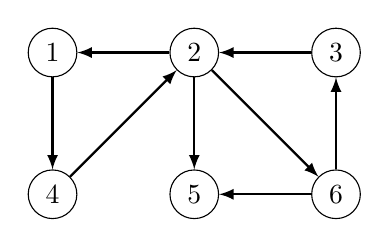
\begin{tikzpicture}[scale=0.9]
\node[draw, circle] (1) at (1,3) {$1$};
\node[draw, circle] (2) at (1,1) {$4$};
\node[draw, circle] (3) at (3,3) {$2$};
\node[draw, circle] (4) at (5,3) {$3$};
\node[draw, circle] (5) at (3,1) {$5$};
\node[draw, circle] (6) at (5,1) {$6$};

\path[draw,thick,->,>=latex] (1) -- (2);
\path[draw,thick,->,>=latex] (2) -- (3);
\path[draw,thick,->,>=latex] (3) -- (1);
\path[draw,thick,->,>=latex] (4) -- (3);
\path[draw,thick,->,>=latex] (3) -- (5);
\path[draw,thick,->,>=latex] (3) -- (6);
\path[draw,thick,->,>=latex] (6) -- (4);
\path[draw,thick,->,>=latex] (6) -- (5);
\end{tikzpicture}
\end{center}

vierusmatriisi on

\[
V=
\left( \begin{array}{cccccc}
0 & 0 & 0 & 1 & 0 & 0 \\
1 & 0 & 0 & 0 & 1 & 1 \\
0 & 1 & 0 & 0 & 0 & 0 \\
0 & 1 & 0 & 0 & 0 & 0 \\
0 & 0 & 0 & 0 & 0 & 0 \\
0 & 0 & 1 & 0 & 1 & 0 \end{array} \right).
\]

Nyt esimerkiksi matriisi $V^3$ kertoo
3:n pituisten polkujen määrät:
\[
V^3=
\left( \begin{array}{cccccc}
1 & 0 & 0 & 0 & 1 & 1 \\
0 & 2 & 0 & 0 & 0 & 0 \\
0 & 0 & 1 & 1 & 1 & 0 \\
0 & 0 & 1 & 1 & 1 & 0 \\
0 & 0 & 0 & 0 & 0 & 0 \\
1 & 0 & 0 & 0 & 1 & 1 \end{array} \right).
\]

Esimerkiksi $(V^3)_{1,5}=1$,
koska solmusta 1 pääsee solmuun 5
kulkemalla polkua $1 \rightarrow 4 \rightarrow 2 \rightarrow 5$.
Vastaavasti $(V^3)_{2,2}=2$,
koska solmusta 2 pääsee itseensä
kulkemalla polkuja
$2 \rightarrow 1 \rightarrow 4 \rightarrow 2$
sekä $2 \rightarrow 6 \rightarrow 3 \rightarrow 2$.

Samantapaista ideaa voi käyttää myös
laskemaan painotetussa verkossa,
mikä on lyhin $k$ kaaren pituinen polku
kunkin solmun välillä.
Tämän saavuttamiseksi riittää muuttaa matriisikertolaskun
kaavassa yhteenlasku minimiksi
ja kertolasku yhteenlaskuksi,
jolloin kaavasta tulee

\[
(AB)_{i,j} = \min_{k=1}^n (A_{i,k}+B_{k,j}).
\]

